
% Default to the notebook output style

    


% Inherit from the specified cell style.




    
\documentclass{article}

    
    
    \usepackage{graphicx} % Used to insert images
    \usepackage{adjustbox} % Used to constrain images to a maximum size 
    \usepackage{color} % Allow colors to be defined
    \usepackage{enumerate} % Needed for markdown enumerations to work
    \usepackage{geometry} % Used to adjust the document margins
    \usepackage{amsmath} % Equations
    \usepackage{amssymb} % Equations
    \usepackage[mathletters]{ucs} % Extended unicode (utf-8) support
    \usepackage[utf8x]{inputenc} % Allow utf-8 characters in the tex document
    \usepackage{fancyvrb} % verbatim replacement that allows latex
    \usepackage{grffile} % extends the file name processing of package graphics 
                         % to support a larger range 
    % The hyperref package gives us a pdf with properly built
    % internal navigation ('pdf bookmarks' for the table of contents,
    % internal cross-reference links, web links for URLs, etc.)
    \usepackage{hyperref}
    \usepackage{longtable} % longtable support required by pandoc >1.10
    \usepackage{booktabs}  % table support for pandoc > 1.12.2
    

    
    
    \definecolor{orange}{cmyk}{0,0.4,0.8,0.2}
    \definecolor{darkorange}{rgb}{.71,0.21,0.01}
    \definecolor{darkgreen}{rgb}{.12,.54,.11}
    \definecolor{myteal}{rgb}{.26, .44, .56}
    \definecolor{gray}{gray}{0.45}
    \definecolor{lightgray}{gray}{.95}
    \definecolor{mediumgray}{gray}{.8}
    \definecolor{inputbackground}{rgb}{.95, .95, .85}
    \definecolor{outputbackground}{rgb}{.95, .95, .95}
    \definecolor{traceback}{rgb}{1, .95, .95}
    % ansi colors
    \definecolor{red}{rgb}{.6,0,0}
    \definecolor{green}{rgb}{0,.65,0}
    \definecolor{brown}{rgb}{0.6,0.6,0}
    \definecolor{blue}{rgb}{0,.145,.698}
    \definecolor{purple}{rgb}{.698,.145,.698}
    \definecolor{cyan}{rgb}{0,.698,.698}
    \definecolor{lightgray}{gray}{0.5}
    
    % bright ansi colors
    \definecolor{darkgray}{gray}{0.25}
    \definecolor{lightred}{rgb}{1.0,0.39,0.28}
    \definecolor{lightgreen}{rgb}{0.48,0.99,0.0}
    \definecolor{lightblue}{rgb}{0.53,0.81,0.92}
    \definecolor{lightpurple}{rgb}{0.87,0.63,0.87}
    \definecolor{lightcyan}{rgb}{0.5,1.0,0.83}
    
    % commands and environments needed by pandoc snippets
    % extracted from the output of `pandoc -s`
    \DefineVerbatimEnvironment{Highlighting}{Verbatim}{commandchars=\\\{\}}
    % Add ',fontsize=\small' for more characters per line
    \newenvironment{Shaded}{}{}
    \newcommand{\KeywordTok}[1]{\textcolor[rgb]{0.00,0.44,0.13}{\textbf{{#1}}}}
    \newcommand{\DataTypeTok}[1]{\textcolor[rgb]{0.56,0.13,0.00}{{#1}}}
    \newcommand{\DecValTok}[1]{\textcolor[rgb]{0.25,0.63,0.44}{{#1}}}
    \newcommand{\BaseNTok}[1]{\textcolor[rgb]{0.25,0.63,0.44}{{#1}}}
    \newcommand{\FloatTok}[1]{\textcolor[rgb]{0.25,0.63,0.44}{{#1}}}
    \newcommand{\CharTok}[1]{\textcolor[rgb]{0.25,0.44,0.63}{{#1}}}
    \newcommand{\StringTok}[1]{\textcolor[rgb]{0.25,0.44,0.63}{{#1}}}
    \newcommand{\CommentTok}[1]{\textcolor[rgb]{0.38,0.63,0.69}{\textit{{#1}}}}
    \newcommand{\OtherTok}[1]{\textcolor[rgb]{0.00,0.44,0.13}{{#1}}}
    \newcommand{\AlertTok}[1]{\textcolor[rgb]{1.00,0.00,0.00}{\textbf{{#1}}}}
    \newcommand{\FunctionTok}[1]{\textcolor[rgb]{0.02,0.16,0.49}{{#1}}}
    \newcommand{\RegionMarkerTok}[1]{{#1}}
    \newcommand{\ErrorTok}[1]{\textcolor[rgb]{1.00,0.00,0.00}{\textbf{{#1}}}}
    \newcommand{\NormalTok}[1]{{#1}}
    
    % Define a nice break command that doesn't care if a line doesn't already
    % exist.
    \def\br{\hspace*{\fill} \\* }
    % Math Jax compatability definitions
    \def\gt{>}
    \def\lt{<}
    % Document parameters
    \title{02\_Speeding\_Python}
    
    
    

    % Pygments definitions
    
\makeatletter
\def\PY@reset{\let\PY@it=\relax \let\PY@bf=\relax%
    \let\PY@ul=\relax \let\PY@tc=\relax%
    \let\PY@bc=\relax \let\PY@ff=\relax}
\def\PY@tok#1{\csname PY@tok@#1\endcsname}
\def\PY@toks#1+{\ifx\relax#1\empty\else%
    \PY@tok{#1}\expandafter\PY@toks\fi}
\def\PY@do#1{\PY@bc{\PY@tc{\PY@ul{%
    \PY@it{\PY@bf{\PY@ff{#1}}}}}}}
\def\PY#1#2{\PY@reset\PY@toks#1+\relax+\PY@do{#2}}

\expandafter\def\csname PY@tok@gd\endcsname{\def\PY@tc##1{\textcolor[rgb]{0.63,0.00,0.00}{##1}}}
\expandafter\def\csname PY@tok@gu\endcsname{\let\PY@bf=\textbf\def\PY@tc##1{\textcolor[rgb]{0.50,0.00,0.50}{##1}}}
\expandafter\def\csname PY@tok@gt\endcsname{\def\PY@tc##1{\textcolor[rgb]{0.00,0.27,0.87}{##1}}}
\expandafter\def\csname PY@tok@gs\endcsname{\let\PY@bf=\textbf}
\expandafter\def\csname PY@tok@gr\endcsname{\def\PY@tc##1{\textcolor[rgb]{1.00,0.00,0.00}{##1}}}
\expandafter\def\csname PY@tok@cm\endcsname{\let\PY@it=\textit\def\PY@tc##1{\textcolor[rgb]{0.25,0.50,0.50}{##1}}}
\expandafter\def\csname PY@tok@vg\endcsname{\def\PY@tc##1{\textcolor[rgb]{0.10,0.09,0.49}{##1}}}
\expandafter\def\csname PY@tok@m\endcsname{\def\PY@tc##1{\textcolor[rgb]{0.40,0.40,0.40}{##1}}}
\expandafter\def\csname PY@tok@mh\endcsname{\def\PY@tc##1{\textcolor[rgb]{0.40,0.40,0.40}{##1}}}
\expandafter\def\csname PY@tok@go\endcsname{\def\PY@tc##1{\textcolor[rgb]{0.53,0.53,0.53}{##1}}}
\expandafter\def\csname PY@tok@ge\endcsname{\let\PY@it=\textit}
\expandafter\def\csname PY@tok@vc\endcsname{\def\PY@tc##1{\textcolor[rgb]{0.10,0.09,0.49}{##1}}}
\expandafter\def\csname PY@tok@il\endcsname{\def\PY@tc##1{\textcolor[rgb]{0.40,0.40,0.40}{##1}}}
\expandafter\def\csname PY@tok@cs\endcsname{\let\PY@it=\textit\def\PY@tc##1{\textcolor[rgb]{0.25,0.50,0.50}{##1}}}
\expandafter\def\csname PY@tok@cp\endcsname{\def\PY@tc##1{\textcolor[rgb]{0.74,0.48,0.00}{##1}}}
\expandafter\def\csname PY@tok@gi\endcsname{\def\PY@tc##1{\textcolor[rgb]{0.00,0.63,0.00}{##1}}}
\expandafter\def\csname PY@tok@gh\endcsname{\let\PY@bf=\textbf\def\PY@tc##1{\textcolor[rgb]{0.00,0.00,0.50}{##1}}}
\expandafter\def\csname PY@tok@ni\endcsname{\let\PY@bf=\textbf\def\PY@tc##1{\textcolor[rgb]{0.60,0.60,0.60}{##1}}}
\expandafter\def\csname PY@tok@nl\endcsname{\def\PY@tc##1{\textcolor[rgb]{0.63,0.63,0.00}{##1}}}
\expandafter\def\csname PY@tok@nn\endcsname{\let\PY@bf=\textbf\def\PY@tc##1{\textcolor[rgb]{0.00,0.00,1.00}{##1}}}
\expandafter\def\csname PY@tok@no\endcsname{\def\PY@tc##1{\textcolor[rgb]{0.53,0.00,0.00}{##1}}}
\expandafter\def\csname PY@tok@na\endcsname{\def\PY@tc##1{\textcolor[rgb]{0.49,0.56,0.16}{##1}}}
\expandafter\def\csname PY@tok@nb\endcsname{\def\PY@tc##1{\textcolor[rgb]{0.00,0.50,0.00}{##1}}}
\expandafter\def\csname PY@tok@nc\endcsname{\let\PY@bf=\textbf\def\PY@tc##1{\textcolor[rgb]{0.00,0.00,1.00}{##1}}}
\expandafter\def\csname PY@tok@nd\endcsname{\def\PY@tc##1{\textcolor[rgb]{0.67,0.13,1.00}{##1}}}
\expandafter\def\csname PY@tok@ne\endcsname{\let\PY@bf=\textbf\def\PY@tc##1{\textcolor[rgb]{0.82,0.25,0.23}{##1}}}
\expandafter\def\csname PY@tok@nf\endcsname{\def\PY@tc##1{\textcolor[rgb]{0.00,0.00,1.00}{##1}}}
\expandafter\def\csname PY@tok@si\endcsname{\let\PY@bf=\textbf\def\PY@tc##1{\textcolor[rgb]{0.73,0.40,0.53}{##1}}}
\expandafter\def\csname PY@tok@s2\endcsname{\def\PY@tc##1{\textcolor[rgb]{0.73,0.13,0.13}{##1}}}
\expandafter\def\csname PY@tok@vi\endcsname{\def\PY@tc##1{\textcolor[rgb]{0.10,0.09,0.49}{##1}}}
\expandafter\def\csname PY@tok@nt\endcsname{\let\PY@bf=\textbf\def\PY@tc##1{\textcolor[rgb]{0.00,0.50,0.00}{##1}}}
\expandafter\def\csname PY@tok@nv\endcsname{\def\PY@tc##1{\textcolor[rgb]{0.10,0.09,0.49}{##1}}}
\expandafter\def\csname PY@tok@s1\endcsname{\def\PY@tc##1{\textcolor[rgb]{0.73,0.13,0.13}{##1}}}
\expandafter\def\csname PY@tok@sh\endcsname{\def\PY@tc##1{\textcolor[rgb]{0.73,0.13,0.13}{##1}}}
\expandafter\def\csname PY@tok@sc\endcsname{\def\PY@tc##1{\textcolor[rgb]{0.73,0.13,0.13}{##1}}}
\expandafter\def\csname PY@tok@sx\endcsname{\def\PY@tc##1{\textcolor[rgb]{0.00,0.50,0.00}{##1}}}
\expandafter\def\csname PY@tok@bp\endcsname{\def\PY@tc##1{\textcolor[rgb]{0.00,0.50,0.00}{##1}}}
\expandafter\def\csname PY@tok@c1\endcsname{\let\PY@it=\textit\def\PY@tc##1{\textcolor[rgb]{0.25,0.50,0.50}{##1}}}
\expandafter\def\csname PY@tok@kc\endcsname{\let\PY@bf=\textbf\def\PY@tc##1{\textcolor[rgb]{0.00,0.50,0.00}{##1}}}
\expandafter\def\csname PY@tok@c\endcsname{\let\PY@it=\textit\def\PY@tc##1{\textcolor[rgb]{0.25,0.50,0.50}{##1}}}
\expandafter\def\csname PY@tok@mf\endcsname{\def\PY@tc##1{\textcolor[rgb]{0.40,0.40,0.40}{##1}}}
\expandafter\def\csname PY@tok@err\endcsname{\def\PY@bc##1{\setlength{\fboxsep}{0pt}\fcolorbox[rgb]{1.00,0.00,0.00}{1,1,1}{\strut ##1}}}
\expandafter\def\csname PY@tok@kd\endcsname{\let\PY@bf=\textbf\def\PY@tc##1{\textcolor[rgb]{0.00,0.50,0.00}{##1}}}
\expandafter\def\csname PY@tok@ss\endcsname{\def\PY@tc##1{\textcolor[rgb]{0.10,0.09,0.49}{##1}}}
\expandafter\def\csname PY@tok@sr\endcsname{\def\PY@tc##1{\textcolor[rgb]{0.73,0.40,0.53}{##1}}}
\expandafter\def\csname PY@tok@mo\endcsname{\def\PY@tc##1{\textcolor[rgb]{0.40,0.40,0.40}{##1}}}
\expandafter\def\csname PY@tok@kn\endcsname{\let\PY@bf=\textbf\def\PY@tc##1{\textcolor[rgb]{0.00,0.50,0.00}{##1}}}
\expandafter\def\csname PY@tok@mi\endcsname{\def\PY@tc##1{\textcolor[rgb]{0.40,0.40,0.40}{##1}}}
\expandafter\def\csname PY@tok@gp\endcsname{\let\PY@bf=\textbf\def\PY@tc##1{\textcolor[rgb]{0.00,0.00,0.50}{##1}}}
\expandafter\def\csname PY@tok@o\endcsname{\def\PY@tc##1{\textcolor[rgb]{0.40,0.40,0.40}{##1}}}
\expandafter\def\csname PY@tok@kr\endcsname{\let\PY@bf=\textbf\def\PY@tc##1{\textcolor[rgb]{0.00,0.50,0.00}{##1}}}
\expandafter\def\csname PY@tok@s\endcsname{\def\PY@tc##1{\textcolor[rgb]{0.73,0.13,0.13}{##1}}}
\expandafter\def\csname PY@tok@kp\endcsname{\def\PY@tc##1{\textcolor[rgb]{0.00,0.50,0.00}{##1}}}
\expandafter\def\csname PY@tok@w\endcsname{\def\PY@tc##1{\textcolor[rgb]{0.73,0.73,0.73}{##1}}}
\expandafter\def\csname PY@tok@kt\endcsname{\def\PY@tc##1{\textcolor[rgb]{0.69,0.00,0.25}{##1}}}
\expandafter\def\csname PY@tok@ow\endcsname{\let\PY@bf=\textbf\def\PY@tc##1{\textcolor[rgb]{0.67,0.13,1.00}{##1}}}
\expandafter\def\csname PY@tok@sb\endcsname{\def\PY@tc##1{\textcolor[rgb]{0.73,0.13,0.13}{##1}}}
\expandafter\def\csname PY@tok@k\endcsname{\let\PY@bf=\textbf\def\PY@tc##1{\textcolor[rgb]{0.00,0.50,0.00}{##1}}}
\expandafter\def\csname PY@tok@se\endcsname{\let\PY@bf=\textbf\def\PY@tc##1{\textcolor[rgb]{0.73,0.40,0.13}{##1}}}
\expandafter\def\csname PY@tok@sd\endcsname{\let\PY@it=\textit\def\PY@tc##1{\textcolor[rgb]{0.73,0.13,0.13}{##1}}}

\def\PYZbs{\char`\\}
\def\PYZus{\char`\_}
\def\PYZob{\char`\{}
\def\PYZcb{\char`\}}
\def\PYZca{\char`\^}
\def\PYZam{\char`\&}
\def\PYZlt{\char`\<}
\def\PYZgt{\char`\>}
\def\PYZsh{\char`\#}
\def\PYZpc{\char`\%}
\def\PYZdl{\char`\$}
\def\PYZhy{\char`\-}
\def\PYZsq{\char`\'}
\def\PYZdq{\char`\"}
\def\PYZti{\char`\~}
% for compatibility with earlier versions
\def\PYZat{@}
\def\PYZlb{[}
\def\PYZrb{]}
\makeatother


    % Exact colors from NB
    \definecolor{incolor}{rgb}{0.0, 0.0, 0.5}
    \definecolor{outcolor}{rgb}{0.545, 0.0, 0.0}



    
    % Prevent overflowing lines due to hard-to-break entities
    \sloppy 
    % Setup hyperref package
    \hypersetup{
      breaklinks=true,  % so long urls are correctly broken across lines
      colorlinks=true,
      urlcolor=blue,
      linkcolor=darkorange,
      citecolor=darkgreen,
      }
    % Slightly bigger margins than the latex defaults
    
    \geometry{verbose,tmargin=1in,bmargin=1in,lmargin=1in,rmargin=1in}
    
    

    \begin{document}
    
    
    \maketitle
    
    

    
    \section{Speeding Python}\label{speeding-python}

\section{Python in HPC Tutorial}\label{python-in-hpc-tutorial}

\subsection{Supercomputing 2014}\label{supercomputing-2014}

Matt Knepley and Aron Ahmadia

\href{http://creativecommons.org/licenses/by/3.0/deed.en_US}{
\includegraphics{./files/figures/creative_commons_logo.png}}

    \begin{center}\rule{3in}{0.4pt}\end{center}

\subsection{About This Tutorial}\label{about-this-tutorial}

\subsubsection{PyHPC Tutorial on GitHub}\label{pyhpc-tutorial-on-github}

These presentation materials are part of a continuously updated tutorial
on Python for High Performance Computing. Future versions of this
presentation will be found at:

https://github.com/pyhpc/pyhpc-tutorial

Please set all permanent bookmarks to this URL.

\subsubsection{}\label{section}

Checkout from git

\begin{verbatim}
git clone https://github.com/pyhpc/pyhpc-tutorial.git
git checkout sahpc2012
\end{verbatim}

\subsubsection{Viewing the read-only version of this presentation on
nbviewer:}\label{viewing-the-read-only-version-of-this-presentation-on-nbviewer}

\begin{itemize}
\itemsep1pt\parskip0pt\parsep0pt
\item
  \url{http://nbviewer.ipython.org/urls/raw.github.com/pyhpc/pyhpc-tutorial/master/notebooks/02\_Speeding\_Python.ipynb}
\end{itemize}

    \begin{center}\rule{3in}{0.4pt}\end{center}

\subsection{Interacting with the Tutorial
Slides}\label{interacting-with-the-tutorial-slides}

This tutorial is an interactive worksheet designed to encourage you to
try out the lessons during the demonstration. If you are looking at the
PDF version of these slides, we encourage you to download the updated
version (see previous slide) and try the interactive version.

To run the interactive version of this notebook, you will need a Python
2.7 environment including:

\begin{itemize}
\itemsep1pt\parskip0pt\parsep0pt
\item
  IPython version \textgreater{}= 13.0
\item
  numpy version \textgreater{}= 1.6
\item
  scipy \textgreater{}= 0.10
\item
  matplotlib \textgreater{}= 1.0.0
\end{itemize}

Move to the directory containing the tarball and execute:

\begin{verbatim}
$ ipython notebook --pylab=inline
\end{verbatim}

If you are installing the packages yourself, Continuum Analytics
provides both free community as well as professional versions of the
Anaconda installer, which provides all the packages you will need for
this portion of the tutorial. The installer is available from the
\href{https://store.continuum.io/cshop/anaconda}{Anaconda download page
at Continuum Analytics}.

You are also welcome to use Enthought's Python Distribution (free for
Academic users), available from the
\href{http://www.enthought.com/products/epd.php}{EPD download page at
Enthought}.


    \begin{center}\rule{3in}{0.4pt}\end{center}

\subsection{How Slow is Python}\label{how-slow-is-python}

Let's add one to a million number

    \begin{Verbatim}[commandchars=\\\{\}]
{\color{incolor}In [{\color{incolor}2}]:} \PY{n}{lst} \PY{o}{=} \PY{n+nb}{range}\PY{p}{(}\PY{l+m+mi}{1000000}\PY{p}{)} \PY{c}{\PYZsh{} A pure Python list}
        \PY{o}{\PYZpc{}}\PY{k}{timeit} \PY{p}{[}\PY{n}{i} \PY{o}{+} \PY{l+m+mi}{1} \PY{k}{for} \PY{n}{i} \PY{o+ow}{in} \PY{n}{lst}\PY{p}{]} 
        \PY{c}{\PYZsh{} A Python list comprehension (iteration happens in C but with PyObjects)}
\end{Verbatim}

    \begin{Verbatim}[commandchars=\\\{\}]
1 loops, best of 3: 194 ms per loop
    \end{Verbatim}

    \begin{center}\rule{3in}{0.4pt}\end{center}

\subsection{Why is Python Slow?}\label{why-is-python-slow}

Dynamic typing requires lots of metadata around variable.

\begin{itemize}
\itemsep1pt\parskip0pt\parsep0pt
\item
  Python uses heavy frame objects during iteration
\end{itemize}

\subsubsection{Solution:}\label{solution}

\begin{itemize}
\itemsep1pt\parskip0pt\parsep0pt
\item
  Make an object that has a single type and continuous storage.
\item
  Implement common functionality into that object to iterate in C.
\end{itemize}

    \begin{Verbatim}[commandchars=\\\{\}]
{\color{incolor}In [{\color{incolor}3}]:} \PY{n}{arr} \PY{o}{=} \PY{n}{np}\PY{o}{.}\PY{n}{arange}\PY{p}{(}\PY{l+m+mi}{1000000}\PY{p}{)} \PY{c}{\PYZsh{} A NumPy list of integers}
        \PY{o}{\PYZpc{}}\PY{k}{timeit} \PY{n}{arr} \PY{o}{+} \PY{l+m+mi}{1} \PY{c}{\PYZsh{} Use operator overloading for nice syntax, now iteration is in C with ints}
\end{Verbatim}

    \begin{Verbatim}[commandchars=\\\{\}]
100 loops, best of 3: 7.45 ms per loop
    \end{Verbatim}

    \begin{center}\rule{3in}{0.4pt}\end{center}

\subsection{What makes NumPy so much
faster?}\label{what-makes-numpy-so-much-faster}

\begin{itemize}
\item
  Data layout
\item
  homogenous: every item takes up the same size block of memory
\item
  single data-type objects
\item
  powerful array scalar types
\item
  universal function (ufuncs)
\item
  function that operates on ndarrays in an element-by-element fashion
\item
  vectorized wrapper for a function
\item
  built-in functions are implemented in compiled C code
\end{itemize}

    \begin{center}\rule{3in}{0.4pt}\end{center}

\subsection{Numpy Data layout}\label{numpy-data-layout}

\begin{itemize}
\itemsep1pt\parskip0pt\parsep0pt
\item
  homogenous: every item takes up the same size block of memory
\item
  single data-type objects
\item
  powerful array scalar types
\end{itemize}

\begin{figure}[htbp]
\centering
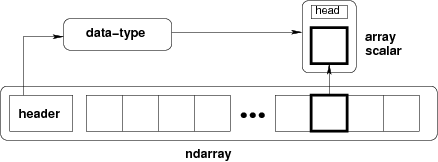
\includegraphics{./files/figures/numpy/threefundamental.png}
\caption{three fundamental}
\end{figure}

    \begin{center}\rule{3in}{0.4pt}\end{center}

\subsection{Numpy Universal Functions
(ufuncs)}\label{numpy-universal-functions-ufuncs}

\begin{itemize}
\itemsep1pt\parskip0pt\parsep0pt
\item
  function that operates on ndarrays in an element-by-element fashion
\item
  vectorized wrapper for a function
\item
  built-in functions are implemented in compiled C code
\end{itemize}

    \begin{Verbatim}[commandchars=\\\{\}]
{\color{incolor}In [{\color{incolor}4}]:} \PY{o}{\PYZpc{}}\PY{k}{timeit} \PY{p}{[}\PY{n}{sin}\PY{p}{(}\PY{n}{i}\PY{p}{)}\PY{o}{*}\PY{o}{*}\PY{l+m+mi}{2} \PY{k}{for} \PY{n}{i} \PY{o+ow}{in} \PY{n}{arr}\PY{p}{]}
\end{Verbatim}

    \begin{Verbatim}[commandchars=\\\{\}]
1 loops, best of 3: 9.08 s per loop
    \end{Verbatim}

    \begin{Verbatim}[commandchars=\\\{\}]
{\color{incolor}In [{\color{incolor}5}]:} \PY{o}{\PYZpc{}}\PY{k}{timeit} \PY{n}{np}\PY{o}{.}\PY{n}{sin}\PY{p}{(}\PY{n}{arr}\PY{p}{)}\PY{o}{*}\PY{o}{*}\PY{l+m+mi}{2}
\end{Verbatim}

    \begin{Verbatim}[commandchars=\\\{\}]
10 loops, best of 3: 58.6 ms per loop
    \end{Verbatim}

    \begin{center}\rule{3in}{0.4pt}\end{center}

\subsection{Other Numpy Features to be aware
of}\label{other-numpy-features-to-be-aware-of}

\begin{itemize}
\itemsep1pt\parskip0pt\parsep0pt
\item
  Reshaping
\end{itemize}

    \begin{Verbatim}[commandchars=\\\{\}]
{\color{incolor}In [{\color{incolor}6}]:} \PY{n}{arr2} \PY{o}{=} \PY{n}{arr}\PY{o}{.}\PY{n}{reshape}\PY{p}{(}\PY{p}{(}\PY{l+m+mi}{10}\PY{p}{,}\PY{l+m+mi}{100000}\PY{p}{)}\PY{p}{)}
        \PY{k}{print}\PY{p}{(}\PY{n}{arr2}\PY{p}{)}
\end{Verbatim}

    \begin{Verbatim}[commandchars=\\\{\}]
[[     0      1      2 \ldots,  99997  99998  99999]
 [100000 100001 100002 \ldots, 199997 199998 199999]
 [200000 200001 200002 \ldots, 299997 299998 299999]
 \ldots, 
 [700000 700001 700002 \ldots, 799997 799998 799999]
 [800000 800001 800002 \ldots, 899997 899998 899999]
 [900000 900001 900002 \ldots, 999997 999998 999999]]
    \end{Verbatim}

    \begin{itemize}
\itemsep1pt\parskip0pt\parsep0pt
\item
  Memory Views
\end{itemize}

    \begin{Verbatim}[commandchars=\\\{\}]
{\color{incolor}In [{\color{incolor}7}]:} \PY{n}{arr2}\PY{o}{.}\PY{n}{view}\PY{err}{?}
\end{Verbatim}

    \begin{itemize}
\itemsep1pt\parskip0pt\parsep0pt
\item
  Index Slicing
\end{itemize}

    \begin{Verbatim}[commandchars=\\\{\}]
{\color{incolor}In [{\color{incolor}8}]:} \PY{n}{x} \PY{o}{=} \PY{n}{np}\PY{o}{.}\PY{n}{arange}\PY{p}{(}\PY{l+m+mi}{0}\PY{p}{,} \PY{l+m+mi}{20}\PY{p}{,} \PY{l+m+mi}{2}\PY{p}{)}\PY{p}{;} \PY{n}{y} \PY{o}{=} \PY{n}{x}\PY{o}{*}\PY{o}{*}\PY{l+m+mi}{2}
        \PY{p}{(}\PY{p}{(}\PY{n}{y}\PY{p}{[}\PY{l+m+mi}{1}\PY{p}{:}\PY{p}{]} \PY{o}{\PYZhy{}} \PY{n}{y}\PY{p}{[}\PY{p}{:}\PY{o}{\PYZhy{}}\PY{l+m+mi}{1}\PY{p}{]}\PY{p}{)} \PY{o}{/} \PY{p}{(}\PY{n}{x}\PY{p}{[}\PY{l+m+mi}{1}\PY{p}{:}\PY{p}{]} \PY{o}{\PYZhy{}} \PY{n}{x}\PY{p}{[}\PY{p}{:}\PY{o}{\PYZhy{}}\PY{l+m+mi}{1}\PY{p}{]}\PY{p}{)}\PY{p}{)} \PY{c}{\PYZsh{} dy/dx}
\end{Verbatim}

            \begin{Verbatim}[commandchars=\\\{\}]
{\color{outcolor}Out[{\color{outcolor}8}]:} array([ 2,  6, 10, 14, 18, 22, 26, 30, 34])
\end{Verbatim}
        
    \begin{itemize}
\itemsep1pt\parskip0pt\parsep0pt
\item
  Fancy Indexing
\end{itemize}

    \begin{Verbatim}[commandchars=\\\{\}]
{\color{incolor}In [{\color{incolor}9}]:} \PY{n}{evens} \PY{o}{=} \PY{n}{arr}\PY{p}{[}\PY{n}{arr}\PY{o}{\PYZpc{}}\PY{k}{2} \PY{o}{==} \PY{l+m+mi}{0}\PY{p}{]}
        \PY{k}{print}\PY{p}{(}\PY{n}{evens}\PY{p}{)}
\end{Verbatim}

    \begin{Verbatim}[commandchars=\\\{\}]
[     0      2      4 \ldots, 999994 999996 999998]
    \end{Verbatim}

    \begin{center}\rule{3in}{0.4pt}\end{center}

\subsection{Compiling to C}\label{compiling-to-c}

C is faster, and Python is easier to write. We want both!

\subsection{Cython}\label{cython}

\begin{itemize}
\itemsep1pt\parskip0pt\parsep0pt
\item
  a programming language based on Python
\item
  uses extra syntax allowing for optional static type declarations
\item
  source code gets translated into optimized C/C++ code and compiled as
  Python extension modules
\end{itemize}

    \begin{center}\rule{3in}{0.4pt}\end{center}

\subsection{Using Cython in IPython}\label{using-cython-in-ipython}

In IPython we can make any cell call out to Cython via the cell magic.
The user must first install Cython

\begin{verbatim}
$ pip install cython
\end{verbatim}

Then load the extension

    \begin{Verbatim}[commandchars=\\\{\}]
{\color{incolor}In [{\color{incolor}7}]:} \PY{o}{\PYZpc{}}\PY{k}{load\PYZus{}ext} \PY{n}{cythonmagic}
\end{Verbatim}

    Now use \texttt{\%\%cython} at the begining of a code cell to call out
to Cython.

    \begin{Verbatim}[commandchars=\\\{\}]
{\color{incolor}In [{\color{incolor}8}]:} \PY{o}{\PYZpc{}\PYZpc{}}\PY{k}{cython}
        \PY{k}{def} \PY{n+nf}{f\PYZus{}cython}\PY{p}{(}\PY{n+nb}{int} \PY{n}{i}\PY{p}{)}\PY{p}{:}
            \PY{k}{return} \PY{n}{i}\PY{o}{*}\PY{o}{*}\PY{l+m+mi}{4} \PY{o}{+} \PY{l+m+mi}{3}\PY{o}{*}\PY{n}{i}\PY{o}{*}\PY{o}{*}\PY{l+m+mi}{2} \PY{o}{+} \PY{l+m+mi}{10}
\end{Verbatim}

    Now use Cython function in code:

    \begin{Verbatim}[commandchars=\\\{\}]
{\color{incolor}In [{\color{incolor}9}]:} \PY{n}{f\PYZus{}cython}\PY{p}{(}\PY{l+m+mi}{100}\PY{p}{)}
\end{Verbatim}

            \begin{Verbatim}[commandchars=\\\{\}]
{\color{outcolor}Out[{\color{outcolor}9}]:} 100030010
\end{Verbatim}
        
    \begin{center}\rule{3in}{0.4pt}\end{center}

\subsection{How much faster is Cython?}\label{how-much-faster-is-cython}

The more you are able to provide type information the better the
compile. For example f without type information:

    \begin{Verbatim}[commandchars=\\\{\}]
{\color{incolor}In [{\color{incolor}10}]:} \PY{o}{\PYZpc{}\PYZpc{}}\PY{k}{cython}
         \PY{k}{def} \PY{n+nf}{f\PYZus{}slow}\PY{p}{(}\PY{n}{i}\PY{p}{)}\PY{p}{:}
             \PY{k}{return} \PY{n}{i}\PY{o}{*}\PY{o}{*}\PY{l+m+mi}{4} \PY{o}{+} \PY{l+m+mi}{3}\PY{o}{*}\PY{n}{i}\PY{o}{*}\PY{o}{*}\PY{l+m+mi}{2} \PY{o}{+} \PY{l+m+mi}{10}
\end{Verbatim}

    \begin{Verbatim}[commandchars=\\\{\}]
{\color{incolor}In [{\color{incolor}11}]:} \PY{o}{\PYZpc{}}\PY{k}{timeit} \PY{n}{f\PYZus{}slow}\PY{p}{(}\PY{l+m+mi}{100}\PY{p}{)}
\end{Verbatim}

    \begin{Verbatim}[commandchars=\\\{\}]
1000000 loops, best of 3: 356 ns per loop
    \end{Verbatim}

    \begin{Verbatim}[commandchars=\\\{\}]
{\color{incolor}In [{\color{incolor}12}]:} \PY{o}{\PYZpc{}}\PY{k}{timeit} \PY{n}{f\PYZus{}cython}\PY{p}{(}\PY{l+m+mi}{100}\PY{p}{)}
\end{Verbatim}

    \begin{Verbatim}[commandchars=\\\{\}]
10000000 loops, best of 3: 121 ns per loop
    \end{Verbatim}

    \begin{center}\rule{3in}{0.4pt}\end{center}

\subsection{Declaring Cython variables for C
level}\label{declaring-cython-variables-for-c-level}

If you use a variable or function only at the Cython level you can keep
it in C via \texttt{cdef}:

    \begin{Verbatim}[commandchars=\\\{\}]
{\color{incolor}In [{\color{incolor}13}]:} \PY{o}{\PYZpc{}\PYZpc{}}\PY{k}{cython}
         \PY{n}{cdef} \PY{n}{f}\PY{p}{(}\PY{n}{double} \PY{n}{x}\PY{p}{)}\PY{p}{:}
             \PY{k}{return} \PY{n}{x}\PY{o}{*}\PY{o}{*}\PY{l+m+mi}{2}\PY{o}{\PYZhy{}}\PY{n}{x}
         
         \PY{k}{def} \PY{n+nf}{integrate\PYZus{}f}\PY{p}{(}\PY{n}{double} \PY{n}{a}\PY{p}{,} \PY{n}{double} \PY{n}{b}\PY{p}{,} \PY{n+nb}{int} \PY{n}{N}\PY{p}{)}\PY{p}{:}
             \PY{n}{cdef} \PY{n+nb}{int} \PY{n}{i}
             \PY{n}{cdef} \PY{n}{double} \PY{n}{s}\PY{p}{,} \PY{n}{dx}
             \PY{n}{s} \PY{o}{=} \PY{l+m+mi}{0}
             \PY{n}{dx} \PY{o}{=} \PY{p}{(}\PY{n}{b}\PY{o}{\PYZhy{}}\PY{n}{a}\PY{p}{)}\PY{o}{/}\PY{n}{N}
             \PY{k}{for} \PY{n}{i} \PY{o+ow}{in} \PY{n+nb}{range}\PY{p}{(}\PY{n}{N}\PY{p}{)}\PY{p}{:}
                 \PY{n}{s} \PY{o}{+}\PY{o}{=} \PY{n}{f}\PY{p}{(}\PY{n}{a}\PY{o}{+}\PY{n}{i}\PY{o}{*}\PY{n}{dx}\PY{p}{)}
             \PY{k}{return} \PY{n}{s} \PY{o}{*} \PY{n}{dx}
\end{Verbatim}

    \begin{Verbatim}[commandchars=\\\{\}]
{\color{incolor}In [{\color{incolor}14}]:} \PY{o}{\PYZpc{}}\PY{k}{timeit} \PY{n}{integrate\PYZus{}f}\PY{p}{(}\PY{l+m+mf}{1.0}\PY{p}{,} \PY{l+m+mf}{2.0}\PY{p}{,} \PY{l+m+mi}{1000}\PY{p}{)}
\end{Verbatim}

    \begin{Verbatim}[commandchars=\\\{\}]
10000 loops, best of 3: 57.1 µs per loop
    \end{Verbatim}

    The pure Python version:

    \begin{Verbatim}[commandchars=\\\{\}]
{\color{incolor}In [{\color{incolor}15}]:} \PY{k}{def} \PY{n+nf}{f}\PY{p}{(}\PY{n}{x}\PY{p}{)}\PY{p}{:}
             \PY{k}{return} \PY{n}{x}\PY{o}{*}\PY{o}{*}\PY{l+m+mi}{2}\PY{o}{\PYZhy{}}\PY{n}{x}
         
         \PY{k}{def} \PY{n+nf}{integrate\PYZus{}f}\PY{p}{(}\PY{n}{a}\PY{p}{,} \PY{n}{b}\PY{p}{,} \PY{n}{N}\PY{p}{)}\PY{p}{:}
             \PY{n}{s} \PY{o}{=} \PY{l+m+mi}{0}
             \PY{n}{dx} \PY{o}{=} \PY{p}{(}\PY{n}{b}\PY{o}{\PYZhy{}}\PY{n}{a}\PY{p}{)}\PY{o}{/}\PY{n}{N}
             \PY{k}{for} \PY{n}{i} \PY{o+ow}{in} \PY{n+nb}{range}\PY{p}{(}\PY{n}{N}\PY{p}{)}\PY{p}{:}
                 \PY{n}{s} \PY{o}{+}\PY{o}{=} \PY{n}{f}\PY{p}{(}\PY{n}{a}\PY{o}{+}\PY{n}{i}\PY{o}{*}\PY{n}{dx}\PY{p}{)}
             \PY{k}{return} \PY{n}{s} \PY{o}{*} \PY{n}{dx}
\end{Verbatim}

    \begin{Verbatim}[commandchars=\\\{\}]
{\color{incolor}In [{\color{incolor}16}]:} \PY{o}{\PYZpc{}}\PY{k}{timeit} \PY{n}{integrate\PYZus{}f}\PY{p}{(}\PY{l+m+mf}{1.0}\PY{p}{,} \PY{l+m+mf}{2.0}\PY{p}{,} \PY{l+m+mi}{1000}\PY{p}{)}
\end{Verbatim}

    \begin{Verbatim}[commandchars=\\\{\}]
1000 loops, best of 3: 604 µs per loop
    \end{Verbatim}

    \begin{center}\rule{3in}{0.4pt}\end{center}

\subsection{Using NumPy with Cython}\label{using-numpy-with-cython}

You can also use fast accessors to NumPy arrays from Cython:

    \begin{Verbatim}[commandchars=\\\{\}]
{\color{incolor}In [{\color{incolor}17}]:} \PY{o}{\PYZpc{}\PYZpc{}}\PY{k}{cython}
         \PY{k+kn}{import} \PY{n+nn}{numpy} \PY{k+kn}{as} \PY{n+nn}{np}
         \PY{c}{\PYZsh{} \PYZdq{}cimport\PYZdq{} is used to import special compile\PYZhy{}time information}
         \PY{c}{\PYZsh{} about the numpy module (this is stored in a file numpy.pxd which is}
         \PY{c}{\PYZsh{} currently part of the Cython distribution).}
         \PY{n}{cimport} \PY{n}{numpy} \PY{k}{as} \PY{n}{np}
         \PY{c}{\PYZsh{} We now need to fix a datatype for our arrays. I\PYZsq{}ve used the variable}
         \PY{c}{\PYZsh{} DTYPE for this, which is assigned to the usual NumPy runtime}
         \PY{c}{\PYZsh{} type info object.}
         \PY{n}{DTYPE} \PY{o}{=} \PY{n}{np}\PY{o}{.}\PY{n}{int}
         \PY{c}{\PYZsh{} \PYZdq{}ctypedef\PYZdq{} assigns a corresponding compile\PYZhy{}time type to DTYPE\PYZus{}t. For}
         \PY{c}{\PYZsh{} every type in the numpy module there\PYZsq{}s a corresponding compile\PYZhy{}time}
         \PY{c}{\PYZsh{} type with a \PYZus{}t\PYZhy{}suffix.}
         \PY{n}{ctypedef} \PY{n}{np}\PY{o}{.}\PY{n}{int\PYZus{}t} \PY{n}{DTYPE\PYZus{}t}
         \PY{c}{\PYZsh{} \PYZdq{}def\PYZdq{} can type its arguments but not have a return type. The type of the}
         \PY{c}{\PYZsh{} arguments for a \PYZdq{}def\PYZdq{} function is checked at run\PYZhy{}time when entering the}
         \PY{c}{\PYZsh{} function.}
         \PY{c}{\PYZsh{}}
         \PY{c}{\PYZsh{} The arrays f, g and h is typed as \PYZdq{}np.ndarray\PYZdq{} instances. The only effect}
         \PY{c}{\PYZsh{} this has is to a) insert checks that the function arguments really are}
         \PY{c}{\PYZsh{} NumPy arrays, and b) make some attribute access like f.shape[0] much}
         \PY{c}{\PYZsh{} more efficient. (In this example this doesn\PYZsq{}t matter though.)}
         \PY{k}{def} \PY{n+nf}{naive\PYZus{}convolve}\PY{p}{(}\PY{n}{np}\PY{o}{.}\PY{n}{ndarray} \PY{n}{f}\PY{p}{,} \PY{n}{np}\PY{o}{.}\PY{n}{ndarray} \PY{n}{g}\PY{p}{)}\PY{p}{:}
             \PY{k}{if} \PY{n}{g}\PY{o}{.}\PY{n}{shape}\PY{p}{[}\PY{l+m+mi}{0}\PY{p}{]} \PY{o}{\PYZpc{}} \PY{l+m+mi}{2} \PY{o}{!=} \PY{l+m+mi}{1} \PY{o+ow}{or} \PY{n}{g}\PY{o}{.}\PY{n}{shape}\PY{p}{[}\PY{l+m+mi}{1}\PY{p}{]} \PY{o}{\PYZpc{}} \PY{l+m+mi}{2} \PY{o}{!=} \PY{l+m+mi}{1}\PY{p}{:}
                 \PY{k}{raise} \PY{n+ne}{ValueError}\PY{p}{(}\PY{l+s}{\PYZdq{}}\PY{l+s}{Only odd dimensions on filter supported}\PY{l+s}{\PYZdq{}}\PY{p}{)}
             \PY{k}{assert} \PY{n}{f}\PY{o}{.}\PY{n}{dtype} \PY{o}{==} \PY{n}{DTYPE} \PY{o+ow}{and} \PY{n}{g}\PY{o}{.}\PY{n}{dtype} \PY{o}{==} \PY{n}{DTYPE}
             \PY{c}{\PYZsh{} The \PYZdq{}cdef\PYZdq{} keyword is also used within functions to type variables. It}
             \PY{c}{\PYZsh{} can only be used at the top indendation level (there are non\PYZhy{}trivial}
             \PY{c}{\PYZsh{} problems with allowing them in other places, though we\PYZsq{}d love to see}
             \PY{c}{\PYZsh{} good and thought out proposals for it).}
             \PY{c}{\PYZsh{}}
             \PY{c}{\PYZsh{} For the indices, the \PYZdq{}int\PYZdq{} type is used. This corresponds to a C int,}
             \PY{c}{\PYZsh{} other C types (like \PYZdq{}unsigned int\PYZdq{}) could have been used instead.}
             \PY{c}{\PYZsh{} Purists could use \PYZdq{}Py\PYZus{}ssize\PYZus{}t\PYZdq{} which is the proper Python type for}
             \PY{c}{\PYZsh{} array indices.}
             \PY{n}{cdef} \PY{n+nb}{int} \PY{n}{vmax} \PY{o}{=} \PY{n}{f}\PY{o}{.}\PY{n}{shape}\PY{p}{[}\PY{l+m+mi}{0}\PY{p}{]}
             \PY{n}{cdef} \PY{n+nb}{int} \PY{n}{wmax} \PY{o}{=} \PY{n}{f}\PY{o}{.}\PY{n}{shape}\PY{p}{[}\PY{l+m+mi}{1}\PY{p}{]}
             \PY{n}{cdef} \PY{n+nb}{int} \PY{n}{smax} \PY{o}{=} \PY{n}{g}\PY{o}{.}\PY{n}{shape}\PY{p}{[}\PY{l+m+mi}{0}\PY{p}{]}
             \PY{n}{cdef} \PY{n+nb}{int} \PY{n}{tmax} \PY{o}{=} \PY{n}{g}\PY{o}{.}\PY{n}{shape}\PY{p}{[}\PY{l+m+mi}{1}\PY{p}{]}
             \PY{n}{cdef} \PY{n+nb}{int} \PY{n}{smid} \PY{o}{=} \PY{n}{smax} \PY{o}{/}\PY{o}{/} \PY{l+m+mi}{2}
             \PY{n}{cdef} \PY{n+nb}{int} \PY{n}{tmid} \PY{o}{=} \PY{n}{tmax} \PY{o}{/}\PY{o}{/} \PY{l+m+mi}{2}
             \PY{n}{cdef} \PY{n+nb}{int} \PY{n}{xmax} \PY{o}{=} \PY{n}{vmax} \PY{o}{+} \PY{l+m+mi}{2}\PY{o}{*}\PY{n}{smid}
             \PY{n}{cdef} \PY{n+nb}{int} \PY{n}{ymax} \PY{o}{=} \PY{n}{wmax} \PY{o}{+} \PY{l+m+mi}{2}\PY{o}{*}\PY{n}{tmid}
             \PY{n}{cdef} \PY{n}{np}\PY{o}{.}\PY{n}{ndarray} \PY{n}{h} \PY{o}{=} \PY{n}{np}\PY{o}{.}\PY{n}{zeros}\PY{p}{(}\PY{p}{[}\PY{n}{xmax}\PY{p}{,} \PY{n}{ymax}\PY{p}{]}\PY{p}{,} \PY{n}{dtype}\PY{o}{=}\PY{n}{DTYPE}\PY{p}{)}
             \PY{n}{cdef} \PY{n+nb}{int} \PY{n}{x}\PY{p}{,} \PY{n}{y}\PY{p}{,} \PY{n}{s}\PY{p}{,} \PY{n}{t}\PY{p}{,} \PY{n}{v}\PY{p}{,} \PY{n}{w}
             \PY{c}{\PYZsh{} It is very important to type ALL your variables. You do not get any}
             \PY{c}{\PYZsh{} warnings if not, only much slower code (they are implicitly typed as}
             \PY{c}{\PYZsh{} Python objects).}
             \PY{n}{cdef} \PY{n+nb}{int} \PY{n}{s\PYZus{}from}\PY{p}{,} \PY{n}{s\PYZus{}to}\PY{p}{,} \PY{n}{t\PYZus{}from}\PY{p}{,} \PY{n}{t\PYZus{}to}
             \PY{c}{\PYZsh{} For the value variable, we want to use the same data type as is}
             \PY{c}{\PYZsh{} stored in the array, so we use \PYZdq{}DTYPE\PYZus{}t\PYZdq{} as defined above.}
             \PY{c}{\PYZsh{} NB! An important side\PYZhy{}effect of this is that if \PYZdq{}value\PYZdq{} overflows its}
             \PY{c}{\PYZsh{} datatype size, it will simply wrap around like in C, rather than raise}
             \PY{c}{\PYZsh{} an error like in Python.}
             \PY{n}{cdef} \PY{n}{DTYPE\PYZus{}t} \PY{n}{value}
             \PY{k}{for} \PY{n}{x} \PY{o+ow}{in} \PY{n+nb}{range}\PY{p}{(}\PY{n}{xmax}\PY{p}{)}\PY{p}{:}
                 \PY{k}{for} \PY{n}{y} \PY{o+ow}{in} \PY{n+nb}{range}\PY{p}{(}\PY{n}{ymax}\PY{p}{)}\PY{p}{:}
                     \PY{n}{s\PYZus{}from} \PY{o}{=} \PY{n+nb}{max}\PY{p}{(}\PY{n}{smid} \PY{o}{\PYZhy{}} \PY{n}{x}\PY{p}{,} \PY{o}{\PYZhy{}}\PY{n}{smid}\PY{p}{)}
                     \PY{n}{s\PYZus{}to} \PY{o}{=} \PY{n+nb}{min}\PY{p}{(}\PY{p}{(}\PY{n}{xmax} \PY{o}{\PYZhy{}} \PY{n}{x}\PY{p}{)} \PY{o}{\PYZhy{}} \PY{n}{smid}\PY{p}{,} \PY{n}{smid} \PY{o}{+} \PY{l+m+mi}{1}\PY{p}{)}
                     \PY{n}{t\PYZus{}from} \PY{o}{=} \PY{n+nb}{max}\PY{p}{(}\PY{n}{tmid} \PY{o}{\PYZhy{}} \PY{n}{y}\PY{p}{,} \PY{o}{\PYZhy{}}\PY{n}{tmid}\PY{p}{)}
                     \PY{n}{t\PYZus{}to} \PY{o}{=} \PY{n+nb}{min}\PY{p}{(}\PY{p}{(}\PY{n}{ymax} \PY{o}{\PYZhy{}} \PY{n}{y}\PY{p}{)} \PY{o}{\PYZhy{}} \PY{n}{tmid}\PY{p}{,} \PY{n}{tmid} \PY{o}{+} \PY{l+m+mi}{1}\PY{p}{)}
                     \PY{n}{value} \PY{o}{=} \PY{l+m+mi}{0}
                     \PY{k}{for} \PY{n}{s} \PY{o+ow}{in} \PY{n+nb}{range}\PY{p}{(}\PY{n}{s\PYZus{}from}\PY{p}{,} \PY{n}{s\PYZus{}to}\PY{p}{)}\PY{p}{:}
                         \PY{k}{for} \PY{n}{t} \PY{o+ow}{in} \PY{n+nb}{range}\PY{p}{(}\PY{n}{t\PYZus{}from}\PY{p}{,} \PY{n}{t\PYZus{}to}\PY{p}{)}\PY{p}{:}
                             \PY{n}{v} \PY{o}{=} \PY{n}{x} \PY{o}{\PYZhy{}} \PY{n}{smid} \PY{o}{+} \PY{n}{s}
                             \PY{n}{w} \PY{o}{=} \PY{n}{y} \PY{o}{\PYZhy{}} \PY{n}{tmid} \PY{o}{+} \PY{n}{t}
                             \PY{n}{value} \PY{o}{+}\PY{o}{=} \PY{n}{g}\PY{p}{[}\PY{n}{smid} \PY{o}{\PYZhy{}} \PY{n}{s}\PY{p}{,} \PY{n}{tmid} \PY{o}{\PYZhy{}} \PY{n}{t}\PY{p}{]} \PY{o}{*} \PY{n}{f}\PY{p}{[}\PY{n}{v}\PY{p}{,} \PY{n}{w}\PY{p}{]}
                     \PY{n}{h}\PY{p}{[}\PY{n}{x}\PY{p}{,} \PY{n}{y}\PY{p}{]} \PY{o}{=} \PY{n}{value}
             \PY{k}{return} \PY{n}{h}
\end{Verbatim}

    \begin{Verbatim}[commandchars=\\\{\}]
{\color{incolor}In [{\color{incolor}18}]:} \PY{n}{N}\PY{o}{=}\PY{l+m+mi}{100}
         \PY{n}{f} \PY{o}{=} \PY{n}{np}\PY{o}{.}\PY{n}{arange}\PY{p}{(}\PY{n}{N}\PY{o}{*}\PY{n}{N}\PY{p}{,} \PY{n}{dtype}\PY{o}{=}\PY{n}{np}\PY{o}{.}\PY{n}{int}\PY{p}{)}\PY{o}{.}\PY{n}{reshape}\PY{p}{(}\PY{p}{(}\PY{n}{N}\PY{p}{,}\PY{n}{N}\PY{p}{)}\PY{p}{)}
         \PY{n}{g} \PY{o}{=} \PY{n}{np}\PY{o}{.}\PY{n}{arange}\PY{p}{(}\PY{l+m+mi}{81}\PY{p}{,} \PY{n}{dtype}\PY{o}{=}\PY{n}{np}\PY{o}{.}\PY{n}{int}\PY{p}{)}\PY{o}{.}\PY{n}{reshape}\PY{p}{(}\PY{p}{(}\PY{l+m+mi}{9}\PY{p}{,} \PY{l+m+mi}{9}\PY{p}{)}\PY{p}{)}
         \PY{o}{\PYZpc{}}\PY{k}{timeit} \PY{o}{\PYZhy{}}\PY{n}{n2} \PY{o}{\PYZhy{}}\PY{n}{r3} \PY{n}{naive\PYZus{}convolve}\PY{p}{(}\PY{n}{f}\PY{p}{,} \PY{n}{g}\PY{p}{)}
\end{Verbatim}

    \begin{Verbatim}[commandchars=\\\{\}]
2 loops, best of 3: 2.86 s per loop
    \end{Verbatim}

    \begin{center}\rule{3in}{0.4pt}\end{center}

\section{Numba -- A Python Compiler for Numpy
arrays}\label{numba-a-python-compiler-for-numpy-arrays}

The user must install the Numba packages. If you're not using anaconda,
you will need LLVM with RTTI enabled ( See
https://github.com/llvmpy/llvmpy for the most up-to-date instructions)

First compile LLVM 3.3

\begin{verbatim}
$ wget http://llvm.org/releases/3.3/llvm-3.3.src.tar.gz
$ tar zxvf llvm-3.3.src.tar.gz
$ cd llvm-3.3.src
$ ./configure --enable-optimized --prefix=LLVM_BUILD_DIR
$ # It is recommended to separate the custom build from the default system
$ # package.
$ # Be sure your compiler architecture is same as version of Python you will use
$ #  e.g. -arch i386 or -arch x86_64.  It might be best to be explicit about this.
$ REQUIRES_RTTI=1 make install
\end{verbatim}

Then install llvmpy and numba

\begin{verbatim}
$ LLVM_CONFIG_PATH=LLVM_BUILD_DIR/bin/llvm-config pip install llvmpy numba
\end{verbatim}

    \begin{Verbatim}[commandchars=\\\{\}]
{\color{incolor}In [{\color{incolor}1}]:} \PY{k+kn}{import} \PY{n+nn}{numpy} \PY{k+kn}{as} \PY{n+nn}{np}
        \PY{k+kn}{from} \PY{n+nn}{numba} \PY{k+kn}{import} \PY{n}{autojit}\PY{p}{,} \PY{n}{jit}\PY{p}{,} \PY{n}{double}
\end{Verbatim}

    Numba provides two major decorators: \texttt{jit} and \texttt{autojit}.

The \texttt{jit} decorator returns a compiled version of the function
using the input types and the output types of the function. You can
specify the type using \texttt{out\_type(in\_type, ...)} syntax. Array
inputs can be specified using \texttt{{[}:,:{]}} appended to the type.

The \texttt{autojit} decorator does not require you to specify any
types. It watches for what types you call the function with and infers
the type of the return. If there is a previously compiled version of the
code available it uses it, if not it generates machine code for the
function and then executes that code.

    \begin{Verbatim}[commandchars=\\\{\}]
{\color{incolor}In [{\color{incolor}2}]:} \PY{k}{def} \PY{n+nf}{sum}\PY{p}{(}\PY{n}{arr}\PY{p}{)}\PY{p}{:}
            \PY{n}{M}\PY{p}{,} \PY{n}{N} \PY{o}{=} \PY{n}{arr}\PY{o}{.}\PY{n}{shape}
            \PY{n+nb}{sum} \PY{o}{=} \PY{l+m+mf}{0.0}
            \PY{k}{for} \PY{n}{i} \PY{o+ow}{in} \PY{n+nb}{range}\PY{p}{(}\PY{n}{M}\PY{p}{)}\PY{p}{:}
                \PY{k}{for} \PY{n}{j} \PY{o+ow}{in} \PY{n+nb}{range}\PY{p}{(}\PY{n}{N}\PY{p}{)}\PY{p}{:}
                    \PY{n+nb}{sum} \PY{o}{+}\PY{o}{=} \PY{n}{arr}\PY{p}{[}\PY{n}{i}\PY{p}{,}\PY{n}{j}\PY{p}{]}
            \PY{k}{return} \PY{n+nb}{sum}
        \PY{n}{fastsum} \PY{o}{=} \PY{n}{jit}\PY{p}{(}\PY{l+s}{\PYZsq{}}\PY{l+s}{f8(f8[:,:])}\PY{l+s}{\PYZsq{}}\PY{p}{)}\PY{p}{(}\PY{n+nb}{sum}\PY{p}{)}
        \PY{n}{flexsum} \PY{o}{=} \PY{n}{autojit}\PY{p}{(}\PY{n+nb}{sum}\PY{p}{)}
\end{Verbatim}

    \begin{Verbatim}[commandchars=\\\{\}]
{\color{incolor}In [{\color{incolor}3}]:} \PY{n}{arr2d} \PY{o}{=} \PY{n}{np}\PY{o}{.}\PY{n}{arange}\PY{p}{(}\PY{l+m+mi}{600}\PY{p}{,}\PY{n}{dtype}\PY{o}{=}\PY{n+nb}{float}\PY{p}{)}\PY{o}{.}\PY{n}{reshape}\PY{p}{(}\PY{l+m+mi}{20}\PY{p}{,}\PY{l+m+mi}{30}\PY{p}{)}
        \PY{k}{print} \PY{n+nb}{sum}\PY{p}{(}\PY{n}{arr2d}\PY{p}{)}
        \PY{k}{print} \PY{n}{fastsum}\PY{p}{(}\PY{n}{arr2d}\PY{p}{)}
        \PY{k}{print} \PY{n}{flexsum}\PY{p}{(}\PY{n}{arr2d}\PY{p}{)}
        \PY{k}{print} \PY{n}{flexsum}\PY{p}{(}\PY{n}{arr2d}\PY{o}{.}\PY{n}{astype}\PY{p}{(}\PY{n+nb}{int}\PY{p}{)}\PY{p}{)}
\end{Verbatim}

    \begin{Verbatim}[commandchars=\\\{\}]
179700.0
179700.0
179700.0
179700.0
    \end{Verbatim}

    \begin{Verbatim}[commandchars=\\\{\}]
{\color{incolor}In [{\color{incolor}4}]:} \PY{o}{\PYZpc{}}\PY{k}{timeit} \PY{n+nb}{sum}\PY{p}{(}\PY{n}{arr2d}\PY{p}{)}
\end{Verbatim}

    \begin{Verbatim}[commandchars=\\\{\}]
1000 loops, best of 3: 623 µs per loop
    \end{Verbatim}

    \begin{Verbatim}[commandchars=\\\{\}]
{\color{incolor}In [{\color{incolor}5}]:} \PY{o}{\PYZpc{}}\PY{k}{timeit} \PY{n}{fastsum}\PY{p}{(}\PY{n}{arr2d}\PY{p}{)}
\end{Verbatim}

    \begin{Verbatim}[commandchars=\\\{\}]
1000000 loops, best of 3: 1.75 µs per loop
    \end{Verbatim}

    \begin{Verbatim}[commandchars=\\\{\}]
{\color{incolor}In [{\color{incolor}6}]:} \PY{l+m+mi}{623} \PY{o}{/} \PY{l+m+mf}{1.75} \PY{c}{\PYZsh{} speedup}
\end{Verbatim}

            \begin{Verbatim}[commandchars=\\\{\}]
{\color{outcolor}Out[{\color{outcolor}6}]:} 356.0
\end{Verbatim}
        
    \begin{Verbatim}[commandchars=\\\{\}]
{\color{incolor}In [{\color{incolor}7}]:} \PY{o}{\PYZpc{}}\PY{k}{timeit} \PY{n}{arr2d}\PY{o}{.}\PY{n}{sum}\PY{p}{(}\PY{p}{)} 
\end{Verbatim}

    \begin{Verbatim}[commandchars=\\\{\}]
100000 loops, best of 3: 5.14 µs per loop
    \end{Verbatim}

    \begin{Verbatim}[commandchars=\\\{\}]
{\color{incolor}In [{\color{incolor}8}]:} \PY{l+m+mf}{5.14} \PY{o}{/} \PY{l+m+mf}{1.75} \PY{c}{\PYZsh{} even provides a speedup over general\PYZhy{}purpose NumPy surm}
\end{Verbatim}

            \begin{Verbatim}[commandchars=\\\{\}]
{\color{outcolor}Out[{\color{outcolor}8}]:} 2.937142857142857
\end{Verbatim}
        
    The speed-up is even more pronounced the more inner loops in the code.
Here is an image processing example:

    \begin{Verbatim}[commandchars=\\\{\}]
{\color{incolor}In [{\color{incolor}14}]:} \PY{n+nd}{@jit}\PY{p}{(}\PY{l+s}{\PYZsq{}}\PY{l+s}{void(f8[:,:],f8[:,:],f8[:,:])}\PY{l+s}{\PYZsq{}}\PY{p}{)}
         \PY{k}{def} \PY{n+nf}{filter}\PY{p}{(}\PY{n}{image}\PY{p}{,} \PY{n}{filt}\PY{p}{,} \PY{n}{output}\PY{p}{)}\PY{p}{:}
             \PY{n}{M}\PY{p}{,} \PY{n}{N} \PY{o}{=} \PY{n}{image}\PY{o}{.}\PY{n}{shape}
             \PY{n}{m}\PY{p}{,} \PY{n}{n} \PY{o}{=} \PY{n}{filt}\PY{o}{.}\PY{n}{shape}
             \PY{k}{for} \PY{n}{i} \PY{o+ow}{in} \PY{n+nb}{range}\PY{p}{(}\PY{n}{m}\PY{o}{/}\PY{o}{/}\PY{l+m+mi}{2}\PY{p}{,} \PY{n}{M}\PY{o}{\PYZhy{}}\PY{n}{m}\PY{o}{/}\PY{o}{/}\PY{l+m+mi}{2}\PY{p}{)}\PY{p}{:}
                 \PY{k}{for} \PY{n}{j} \PY{o+ow}{in} \PY{n+nb}{range}\PY{p}{(}\PY{n}{n}\PY{o}{/}\PY{o}{/}\PY{l+m+mi}{2}\PY{p}{,} \PY{n}{N}\PY{o}{\PYZhy{}}\PY{n}{n}\PY{o}{/}\PY{o}{/}\PY{l+m+mi}{2}\PY{p}{)}\PY{p}{:}
                     \PY{n}{result} \PY{o}{=} \PY{l+m+mf}{0.0}
                     \PY{k}{for} \PY{n}{k} \PY{o+ow}{in} \PY{n+nb}{range}\PY{p}{(}\PY{n}{m}\PY{p}{)}\PY{p}{:}
                         \PY{k}{for} \PY{n}{l} \PY{o+ow}{in} \PY{n+nb}{range}\PY{p}{(}\PY{n}{n}\PY{p}{)}\PY{p}{:}
                             \PY{n}{result} \PY{o}{+}\PY{o}{=} \PY{n}{image}\PY{p}{[}\PY{n}{i}\PY{o}{+}\PY{n}{k}\PY{o}{\PYZhy{}}\PY{n}{m}\PY{o}{/}\PY{o}{/}\PY{l+m+mi}{2}\PY{p}{,}\PY{n}{j}\PY{o}{+}\PY{n}{l}\PY{o}{\PYZhy{}}\PY{n}{n}\PY{o}{/}\PY{o}{/}\PY{l+m+mi}{2}\PY{p}{]}\PY{o}{*}\PY{n}{filt}\PY{p}{[}\PY{n}{k}\PY{p}{,} \PY{n}{l}\PY{p}{]}
                     \PY{n}{output}\PY{p}{[}\PY{n}{i}\PY{p}{,}\PY{n}{j}\PY{p}{]} \PY{o}{=} \PY{n}{result}
         
         \PY{k+kn}{from} \PY{n+nn}{scipy.misc} \PY{k+kn}{import} \PY{n}{lena}
         \PY{k+kn}{import} \PY{n+nn}{time}
         \PY{n}{image} \PY{o}{=} \PY{n}{lena}\PY{p}{(}\PY{p}{)}\PY{o}{.}\PY{n}{astype}\PY{p}{(}\PY{l+s}{\PYZsq{}}\PY{l+s}{double}\PY{l+s}{\PYZsq{}}\PY{p}{)}
         \PY{n}{filt} \PY{o}{=} \PY{n}{np}\PY{o}{.}\PY{n}{ones}\PY{p}{(}\PY{p}{(}\PY{l+m+mi}{15}\PY{p}{,}\PY{l+m+mi}{15}\PY{p}{)}\PY{p}{,}\PY{n}{dtype}\PY{o}{=}\PY{l+s}{\PYZsq{}}\PY{l+s}{double}\PY{l+s}{\PYZsq{}}\PY{p}{)}
         \PY{n}{filt} \PY{o}{/}\PY{o}{=} \PY{n}{filt}\PY{o}{.}\PY{n}{sum}\PY{p}{(}\PY{p}{)}
         \PY{n}{output} \PY{o}{=} \PY{n}{image}\PY{o}{.}\PY{n}{copy}\PY{p}{(}\PY{p}{)}
         \PY{n+nb}{filter}\PY{p}{(}\PY{n}{image}\PY{p}{,} \PY{n}{filt}\PY{p}{,} \PY{n}{output}\PY{p}{)}
         \PY{n}{gray}\PY{p}{(}\PY{p}{)}
         \PY{n}{imshow}\PY{p}{(}\PY{n}{output}\PY{p}{)}
         \PY{n}{start} \PY{o}{=} \PY{n}{time}\PY{o}{.}\PY{n}{time}\PY{p}{(}\PY{p}{)}
         \PY{n+nb}{filter}\PY{p}{(}\PY{n}{image}\PY{p}{[}\PY{p}{:}\PY{l+m+mi}{100}\PY{p}{,}\PY{p}{:}\PY{l+m+mi}{100}\PY{p}{]}\PY{p}{,} \PY{n}{filt}\PY{p}{,} \PY{n}{output}\PY{p}{[}\PY{p}{:}\PY{l+m+mi}{100}\PY{p}{,}\PY{p}{:}\PY{l+m+mi}{100}\PY{p}{]}\PY{p}{)}
         \PY{n}{fast} \PY{o}{=} \PY{n}{time}\PY{o}{.}\PY{n}{time}\PY{p}{(}\PY{p}{)} \PY{o}{\PYZhy{}} \PY{n}{start}
         \PY{n}{start} \PY{o}{=} \PY{n}{time}\PY{o}{.}\PY{n}{time}\PY{p}{(}\PY{p}{)}
         \PY{n+nb}{filter}\PY{o}{.}\PY{n}{py\PYZus{}func}\PY{p}{(}\PY{n}{image}\PY{p}{[}\PY{p}{:}\PY{l+m+mi}{100}\PY{p}{,}\PY{p}{:}\PY{l+m+mi}{100}\PY{p}{]}\PY{p}{,} \PY{n}{filt}\PY{p}{,} \PY{n}{output}\PY{p}{[}\PY{p}{:}\PY{l+m+mi}{100}\PY{p}{,}\PY{p}{:}\PY{l+m+mi}{100}\PY{p}{]}\PY{p}{)}
         \PY{n}{slow} \PY{o}{=} \PY{n}{time}\PY{o}{.}\PY{n}{time}\PY{p}{(}\PY{p}{)} \PY{o}{\PYZhy{}} \PY{n}{start}
         \PY{k}{print} \PY{l+s}{\PYZdq{}}\PY{l+s}{Python: }\PY{l+s+si}{\PYZpc{}f}\PY{l+s}{ s; Numba: }\PY{l+s+si}{\PYZpc{}f}\PY{l+s}{ ms; Speed up is }\PY{l+s+si}{\PYZpc{}f}\PY{l+s}{\PYZdq{}} \PY{o}{\PYZpc{}} \PY{p}{(}\PY{n}{slow}\PY{p}{,} \PY{n}{fast}\PY{o}{*}\PY{l+m+mi}{1000}\PY{p}{,} \PY{n}{slow} \PY{o}{/} \PY{n}{fast}\PY{p}{)}
\end{Verbatim}

    \begin{Verbatim}[commandchars=\\\{\}]
Python: 4.389855 s; Numba: 7.434130 ms; Speed up is 590.500176
    \end{Verbatim}

    \begin{center}
    \adjustimage{max size={0.9\linewidth}{0.9\paperheight}}{02_Speeding_Python_files/02_Speeding_Python_55_1.png}
    \end{center}
    { \hspace*{\fill} \\}
    
    You can call Numba-created functions from other Numba-created functions

    \begin{Verbatim}[commandchars=\\\{\}]
{\color{incolor}In [{\color{incolor}28}]:} \PY{n+nd}{@autojit}
         \PY{k}{def} \PY{n+nf}{mandel}\PY{p}{(}\PY{n}{x}\PY{p}{,} \PY{n}{y}\PY{p}{,} \PY{n}{max\PYZus{}iters}\PY{p}{)}\PY{p}{:}
             \PY{l+s+sd}{\PYZdq{}\PYZdq{}\PYZdq{}}
         \PY{l+s+sd}{    Given the real and imaginary parts of a complex number,}
         \PY{l+s+sd}{    determine if it is a candidate for membership in the Mandelbrot}
         \PY{l+s+sd}{    set given a fixed number of iterations.}
         \PY{l+s+sd}{    \PYZdq{}\PYZdq{}\PYZdq{}}
             \PY{n}{i} \PY{o}{=} \PY{l+m+mi}{0}
             \PY{n}{c} \PY{o}{=} \PY{n+nb}{complex}\PY{p}{(}\PY{n}{x}\PY{p}{,} \PY{n}{y}\PY{p}{)}
             \PY{n}{z} \PY{o}{=} \PY{l+m+mf}{0.0j}
             \PY{k}{for} \PY{n}{i} \PY{o+ow}{in} \PY{n+nb}{range}\PY{p}{(}\PY{n}{max\PYZus{}iters}\PY{p}{)}\PY{p}{:}
                 \PY{n}{z} \PY{o}{=} \PY{n}{z}\PY{o}{*}\PY{o}{*}\PY{l+m+mi}{2} \PY{o}{+} \PY{n}{c}
                 \PY{k}{if} \PY{n+nb}{abs}\PY{p}{(}\PY{n}{z}\PY{p}{)}\PY{o}{*}\PY{o}{*}\PY{l+m+mi}{2} \PY{o}{\PYZgt{}}\PY{o}{=} \PY{l+m+mi}{4}\PY{p}{:}
                     \PY{k}{return} \PY{n}{i}
         
             \PY{k}{return} \PY{l+m+mi}{255}
         
         \PY{n+nd}{@autojit}
         \PY{k}{def} \PY{n+nf}{create\PYZus{}fractal}\PY{p}{(}\PY{n}{min\PYZus{}x}\PY{p}{,} \PY{n}{max\PYZus{}x}\PY{p}{,} \PY{n}{min\PYZus{}y}\PY{p}{,} \PY{n}{max\PYZus{}y}\PY{p}{,} \PY{n}{image}\PY{p}{,} \PY{n}{iters}\PY{p}{)}\PY{p}{:}
             \PY{n}{height} \PY{o}{=} \PY{n}{image}\PY{o}{.}\PY{n}{shape}\PY{p}{[}\PY{l+m+mi}{0}\PY{p}{]}
             \PY{n}{width} \PY{o}{=} \PY{n}{image}\PY{o}{.}\PY{n}{shape}\PY{p}{[}\PY{l+m+mi}{1}\PY{p}{]}
         
             \PY{n}{pixel\PYZus{}size\PYZus{}x} \PY{o}{=} \PY{p}{(}\PY{n}{max\PYZus{}x} \PY{o}{\PYZhy{}} \PY{n}{min\PYZus{}x}\PY{p}{)} \PY{o}{/} \PY{n}{width}
             \PY{n}{pixel\PYZus{}size\PYZus{}y} \PY{o}{=} \PY{p}{(}\PY{n}{max\PYZus{}y} \PY{o}{\PYZhy{}} \PY{n}{min\PYZus{}y}\PY{p}{)} \PY{o}{/} \PY{n}{height}
             \PY{k}{for} \PY{n}{x} \PY{o+ow}{in} \PY{n+nb}{range}\PY{p}{(}\PY{n}{width}\PY{p}{)}\PY{p}{:}
                 \PY{n}{real} \PY{o}{=} \PY{n}{min\PYZus{}x} \PY{o}{+} \PY{n}{x} \PY{o}{*} \PY{n}{pixel\PYZus{}size\PYZus{}x}
                 \PY{k}{for} \PY{n}{y} \PY{o+ow}{in} \PY{n+nb}{range}\PY{p}{(}\PY{n}{height}\PY{p}{)}\PY{p}{:}
                     \PY{n}{imag} \PY{o}{=} \PY{n}{min\PYZus{}y} \PY{o}{+} \PY{n}{y} \PY{o}{*} \PY{n}{pixel\PYZus{}size\PYZus{}y}
                     \PY{n}{color} \PY{o}{=} \PY{n}{mandel}\PY{p}{(}\PY{n}{real}\PY{p}{,} \PY{n}{imag}\PY{p}{,} \PY{n}{iters}\PY{p}{)}
                     \PY{n}{image}\PY{p}{[}\PY{n}{y}\PY{p}{,} \PY{n}{x}\PY{p}{]} \PY{o}{=} \PY{n}{color}
         
             \PY{k}{return} \PY{n}{image}
         
         \PY{n}{image} \PY{o}{=} \PY{n}{np}\PY{o}{.}\PY{n}{zeros}\PY{p}{(}\PY{p}{(}\PY{l+m+mi}{500}\PY{p}{,} \PY{l+m+mi}{750}\PY{p}{)}\PY{p}{,} \PY{n}{dtype}\PY{o}{=}\PY{n}{np}\PY{o}{.}\PY{n}{uint8}\PY{p}{)}
         \PY{n}{imshow}\PY{p}{(}\PY{n}{create\PYZus{}fractal}\PY{p}{(}\PY{o}{\PYZhy{}}\PY{l+m+mf}{2.0}\PY{p}{,} \PY{l+m+mf}{1.0}\PY{p}{,} \PY{o}{\PYZhy{}}\PY{l+m+mf}{1.0}\PY{p}{,} \PY{l+m+mf}{1.0}\PY{p}{,} \PY{n}{image}\PY{p}{,} \PY{l+m+mi}{20}\PY{p}{)}\PY{p}{)}
\end{Verbatim}

            \begin{Verbatim}[commandchars=\\\{\}]
{\color{outcolor}Out[{\color{outcolor}28}]:} <matplotlib.image.AxesImage at 0x10790a8d0>
\end{Verbatim}
        
    \begin{center}
    \adjustimage{max size={0.9\linewidth}{0.9\paperheight}}{02_Speeding_Python_files/02_Speeding_Python_57_1.png}
    \end{center}
    { \hspace*{\fill} \\}
    
    \begin{Verbatim}[commandchars=\\\{\}]
{\color{incolor}In [{\color{incolor}16}]:} \PY{o}{\PYZpc{}}\PY{k}{timeit} \PY{n}{create\PYZus{}fractal}\PY{p}{(}\PY{o}{\PYZhy{}}\PY{l+m+mf}{2.0}\PY{p}{,} \PY{l+m+mf}{1.0}\PY{p}{,} \PY{o}{\PYZhy{}}\PY{l+m+mf}{1.0}\PY{p}{,} \PY{l+m+mf}{1.0}\PY{p}{,} \PY{n}{image}\PY{p}{,} \PY{l+m+mi}{20}\PY{p}{)}
\end{Verbatim}

    \begin{Verbatim}[commandchars=\\\{\}]
10 loops, best of 3: 40.2 ms per loop
    \end{Verbatim}

    \begin{Verbatim}[commandchars=\\\{\}]
{\color{incolor}In [{\color{incolor}17}]:} \PY{o}{\PYZpc{}}\PY{k}{timeit} \PY{n}{create\PYZus{}fractal}\PY{o}{.}\PY{n}{py\PYZus{}func}\PY{p}{(}\PY{o}{\PYZhy{}}\PY{l+m+mf}{2.0}\PY{p}{,} \PY{l+m+mf}{1.0}\PY{p}{,} \PY{o}{\PYZhy{}}\PY{l+m+mf}{1.0}\PY{p}{,} \PY{l+m+mf}{1.0}\PY{p}{,} \PY{n}{image}\PY{p}{,} \PY{l+m+mi}{20}\PY{p}{)}
\end{Verbatim}

    \begin{Verbatim}[commandchars=\\\{\}]
1 loops, best of 3: 403 ms per loop
    \end{Verbatim}

    \begin{Verbatim}[commandchars=\\\{\}]
{\color{incolor}In [{\color{incolor}18}]:} \PY{l+m+mi}{403}\PY{o}{/} \PY{l+m+mf}{40.2} \PY{c}{\PYZsh{} speedup of compiling outer\PYZhy{}loop (inner\PYZhy{}loop mandel call is still optimized)}
\end{Verbatim}

            \begin{Verbatim}[commandchars=\\\{\}]
{\color{outcolor}Out[{\color{outcolor}18}]:} 10.024875621890546
\end{Verbatim}
        
    \begin{Verbatim}[commandchars=\\\{\}]

================================================================================
    \end{Verbatim}

    Numba works very well for numerical calculations and infers types for
variables. You can over-ride this inference by passing in a locals
dictionary to the autojit decorator. Notice how the code below shows
both Python object manipulation and native manipulation

    \begin{Verbatim}[commandchars=\\\{\}]
{\color{incolor}In [{\color{incolor}20}]:} \PY{k}{class} \PY{n+nc}{MyClass}\PY{p}{(}\PY{n+nb}{object}\PY{p}{)}\PY{p}{:}
             \PY{k}{def} \PY{n+nf}{mymethod}\PY{p}{(}\PY{n+nb+bp}{self}\PY{p}{,} \PY{n}{arg}\PY{p}{)}\PY{p}{:}
                 \PY{k}{return} \PY{n}{arg} \PY{o}{*} \PY{l+m+mi}{2}
             
         \PY{n+nd}{@autojit}\PY{p}{(}\PY{n+nb}{locals}\PY{o}{=}\PY{n+nb}{dict}\PY{p}{(}\PY{n}{mydouble}\PY{o}{=}\PY{n}{double}\PY{p}{)}\PY{p}{)} \PY{c}{\PYZsh{} specify types for local variables}
         \PY{k}{def} \PY{n+nf}{call\PYZus{}method}\PY{p}{(}\PY{n}{obj}\PY{p}{)}\PY{p}{:}
             \PY{k}{print} \PY{n}{obj}\PY{o}{.}\PY{n}{mymethod}\PY{p}{(}\PY{l+s}{\PYZdq{}}\PY{l+s}{hello}\PY{l+s}{\PYZdq{}}\PY{p}{)}   \PY{c}{\PYZsh{} object result}
             \PY{n}{mydouble} \PY{o}{=} \PY{n}{obj}\PY{o}{.}\PY{n}{mymethod}\PY{p}{(}\PY{l+m+mf}{10.2}\PY{p}{)} \PY{c}{\PYZsh{} native double}
             \PY{k}{print}\PY{p}{(}\PY{n}{mydouble} \PY{o}{*} \PY{l+m+mi}{2}\PY{p}{)}           \PY{c}{\PYZsh{} native multiplication}
             
         \PY{n}{call\PYZus{}method}\PY{p}{(}\PY{n}{MyClass}\PY{p}{(}\PY{p}{)}\PY{p}{)}
\end{Verbatim}

    \begin{Verbatim}[commandchars=\\\{\}]
hellohello

40.8
    \end{Verbatim}

    Complex support is available as well.

    \begin{Verbatim}[commandchars=\\\{\}]
{\color{incolor}In [{\color{incolor}25}]:} \PY{n+nd}{@autojit}
         \PY{k}{def} \PY{n+nf}{complex\PYZus{}support}\PY{p}{(}\PY{n}{real}\PY{p}{,} \PY{n}{imag}\PY{p}{)}\PY{p}{:}
             \PY{n}{c} \PY{o}{=} \PY{n+nb}{complex}\PY{p}{(}\PY{n}{real}\PY{p}{,} \PY{n}{imag}\PY{p}{)}
             \PY{k}{return} \PY{p}{(}\PY{n}{c} \PY{o}{*}\PY{o}{*} \PY{l+m+mi}{2}\PY{p}{)}\PY{o}{.}\PY{n}{conjugate}\PY{p}{(}\PY{p}{)}
         
         \PY{n}{c} \PY{o}{=} \PY{l+m+mf}{2.0} \PY{o}{+} \PY{l+m+mf}{4.0j}
         \PY{n}{complex\PYZus{}support}\PY{p}{(}\PY{n}{c}\PY{o}{.}\PY{n}{real}\PY{p}{,} \PY{n}{c}\PY{o}{.}\PY{n}{imag}\PY{p}{)}\PY{p}{,} \PY{p}{(}\PY{n}{c}\PY{o}{*}\PY{o}{*}\PY{l+m+mi}{2}\PY{p}{)}\PY{o}{.}\PY{n}{conjugate}\PY{p}{(}\PY{p}{)}
\end{Verbatim}

            \begin{Verbatim}[commandchars=\\\{\}]
{\color{outcolor}Out[{\color{outcolor}25}]:} ((-12-16j), (-12-16j))
\end{Verbatim}
        
    The roadmap for Numba includes better error-handling, support for almost
all Python syntax which gets compiled to code that either uses machine
instructions or else the Python library run-time, improved support for
basic types, and the ability to create objects easily.

    The commercial product NumbaPro includes additional features:

\begin{itemize}
\itemsep1pt\parskip0pt\parsep0pt
\item
  ability to create ufuncs (fast-vectorize)
\item
  ability to target the GPU via CUDA
\item
  ability to target multiple-cores\\
\item
  array-expressions (ability to write NumPy-like code that gets
  compiled)
\end{itemize}


    % Add a bibliography block to the postdoc
    
    
    
    \end{document}
